\documentclass[11pt]{article}
\usepackage{geometry} % see geometry.pdf on how to lay out the page. There's lots.
\usepackage{hyperref}
\usepackage{graphicx}
\usepackage{gensymb}
\usepackage[affil-it]{authblk}
\usepackage[toc,page]{appendix}
\usepackage{pifont}
\usepackage{amsmath}
\usepackage{float}
%% \usepackage{draftwatermark}

%% \SetWatermarkText{DRAFT}
%% \SetWatermarkScale{6}
%% \SetWatermarkLightness{0.95}

% \geometry{letter} % or letter or a5paper or ... etc
% \geometry{landscape} % rotated page geometry

% See the ``Article customise'' template for come common customisations

\title{The Design and Construction of a Novel Variable-Geometry Snake-like Input Device}

\author{Robert L. Read
  \thanks{read.robert@gmail.com}
  email: \href{mailto:read.robert@gmail.com}{read.robert@gmail.com}\\
Avinash Baskaran
  \thanks{baskaran.avinash@gmail.com}
  email: \href{mailto:Baskaran.avinash@gmail.com}{baskaran.avinash@gmail.com}
  }
  \affil{Public Invention, an educational non-profit.}


\date{\today}

%%% BEGIN DOCUMENT
\begin{document}

\maketitle

%% \tableofcontents


\nocite{read2018transforming,readtetrahelix}

\nocite{sanderson1996modular}

\nocite{lee1999dynamics}

\nocite{lee2002dynamic}

\nocite{NTRT}

\nocite{TetrobotBook}

\nocite{claypool2012readily}

\nocite{mirletz2014}

\nocite{paul2006}




\begin{abstract}

	Humans are skillful. By building a bio-inspired manipulable snake-like controller that can be molded into a wide variety of shapes, we allow a human controller to telepresently specify complex shapes and shape changes. We constructed a tetrahelix consisting of seven tetrahedron made of adjustable-length members connected via 3D printed Song-Kwon-Kim joints which allow manual changes to the shape of the controller. These changes in length are digitized and organized via an Arduino and transmitted to more power computers where they may specify a shape to be animated or control a robot of similar shape, or simply specify relative positions in Cartesian space. Although this research is basic, we hope it will eventually amplify human control of in vivo mechanical devices such as endoscopes, search-and-rescue robots weaseling into tight spaces, or general purpose tetrobots used for planetary space exploration as suggested by Prof. Sanderson and his students 20 years ago.s

\end{abstract}


\section{Introduction}

Snake-like robots are particularly advantageous due to their ability to adopt varying geometries to navigate curvilinear paths.  They accomplish body undulation as a method of locomotion via . The design and construction of such objects relies on flexible actuation with respect to the field of motion.

  We have developed a biomimetically inspired hand-held input device, the motion of which can be digitally mapped onto the existing control mechansisms of robotic systems of to offer users and operators a direct human-robot interface for control. Snake-like robots are particularly advantageous due to their ability to adopt varying geometries to navigate curvilinear paths. Our device can be manipulated in 3-space to conform to various geometries such that the operation of linear robots in 3-space can be accomplished. while snake-like robots often rely on static control mechanisms or digital path planning, while our controller is capable of being dynamically manipulated by a human operator to provide  intuitive control of these  movements, and is thus a more favorable mechanism to operate snake-like robots. 

  The lightweight, modular nature of the device aid in ease of use, and encourage the replacement of damaged or worn our parts, as any single component can be removed and replaced without the need to alter its overall structure. The TetroCon is isomorphic to a Boerdijk-Coxeter helix, which is composed only of tetrahedra, and is thereby inherently rigid, operating as a physical tensegrity, a stable 3D structure, in which every member is either in tension or compression. Its modularity allows for the augmentation of the structure to suit the needs of each individual application, including extending or reducing the number of tetrahedra in the chain to suit the aspect ratio of the robot being controlled, further improving its universality in robotic control.

\subsection{Motivation}

While digital feedback and control mechanisms are useful due to their considerably greater reaction speed, high degree of autonomy, and dependable performance, there exist many applications in which human input is favorable. The  manipulation of robots capable of non-standard geometric configurations can be accomplished via Ai and machine learning algorithms, however, these can be highly time- and cost- intensive to produce and are not consistently relibale in practice. Provided an intuitive, organic human-robot interface, one can accomplish the task of dynamically modulating the physical configuration of a robot, to control it in a non-standard environment.
We have designed and implemented such an interface [reference video]
\section{Abstract Design}
\subsection{Tretrahelix}

[motivate the choice of a tetrahelix controller structure]


\subsection{Linear Displacement to Cartesian}

[describe the algorithm used by bullet]
           
\subsection{The \textit{Turret} Joint}

We employ a novel spherical joint designed by Song et. al. \cite{song2003spherical}, which serves as an effective method for joining linear sections in a tetrahedral configuration while allowing fixed and defined points of rotation. This joint offers a number of unique advantages that make it uniquely suited to our application; its rounded shape makes it an effective gripping tool for the human hand. The ability to alter the geometry of the hole, rotor and shell allows for customizable limits on the range of motion of the device. Most importantly, its removable, two part construction allows for easy addition or removal of single tetrahedra from the larger device, which in conjunction with the modularity of the tetrahedra, allows for a completely customizeable and arbitrary device.
\subsection{Related Research}

[Summarize prof. Sanderson's work, others? explain why our's is more advantageous]

\section{Method and Embodiment}

\subsection{Linear Potentiometers}
\subsection{3D Printred parts}
\subsection{Microelectronics}
 \begin{enumerate}
 \item Mechanism
 \item Housing
 \item Multiplexing
 \item Wireless communication
 \end{enumerate}

 The controller consists of an array of tetrahedrally arranged linear potentiometers embedded within 3D printed sleeve components, which comprise the device's physical framework. Each linear potentiometer allows for measurements of displacement along a single axis, which allows us to map the movement orientation of each sleeve simply using the analog output of each sensor. Each tetrahedron, groupings of 6 linear potentiometers, forming functional subdividisions of the structure, is provided a voltage input, ground, and signal output chanenel via onboard 8-channel multiplexers mounted to a single sleeve within the corresponding tetrahedron.

 [Discuss printed parts, mechanics and dynamics:]
 A controlled flexibility of an otherwise rigid the device,is provided by a spherical joint, invented by Song, Kwon, and Kim [?], depicted conceptually in (figure?: Song, Kwon, Kim, patent image) and (figure?: Turret Joint Planar Geometry).

\begin{figure}[H]
  \centering
    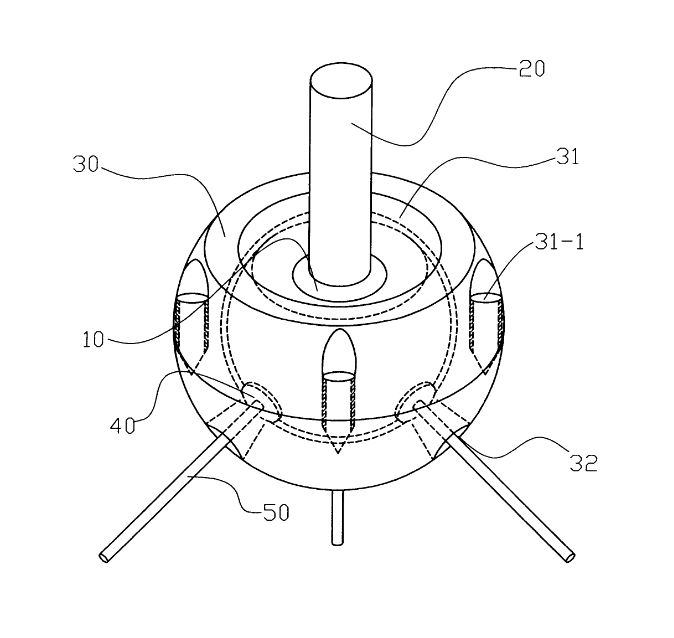
\includegraphics[width=0.5\textwidth]{figures/SongKwonKimImage.png}
    \caption[Song, Kwon, Kim, patent image.]{Song, Kwon, Kim, patent image.}
      \label{SongKwonKimImage}
\end{figure}


\begin{figure}[H]
  \centering
  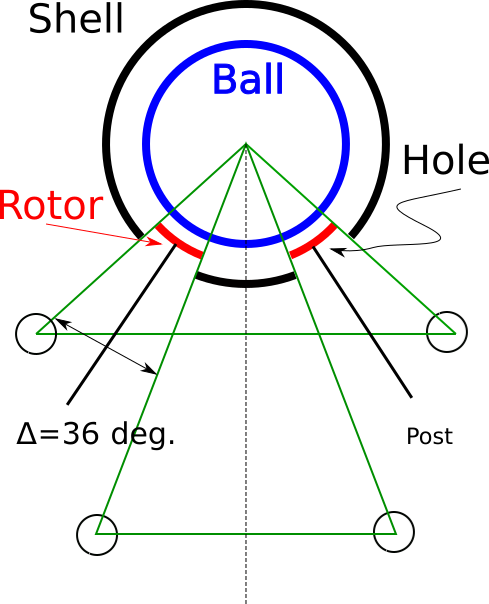
\includegraphics[width=0.5\textwidth]{figures/SimplifiedConstraintDrawing.png}
    \caption[Turret Joint Planar Geometry]{Turret Joint Planar Geometry}
      \label{simplified-constraint-drawing}
\end{figure}

 The  multiplexers send data from the (exact number?) sensors at near real-time to our processing unit, an Arduino Uno microcontroller, which provides 5V supply, ground, analog inputs, and digital control outputs to each of the multiplexers, and streams the data from each sensor via (bluetooth?) to an external location which can create a virtual reconstruction of the device, or further send data to a corresponding robot to be controlled. The use of multiplexers allows the singals from the potentiometers to be read together with little delay time between readings. The result of this system is the ability to precisely match the movement of the controller by a robot receiving the data. We have demonstrated this in (figure?: Screenshot of live visualization of the TetraCon using Dr. Read's software) and in (link?: video of Tetrobot being operated using TetroCon).

\subsection{System Design}
\section{Applications and Uses}
\subsection{Animation and Shaping}
\subsection{Medical Telepresence}

The human body, containing organ systems that are comprised of narrow fluidic channels, is a significant theater of operation for snake-like robots, both in surgical intervention and rehabilitation. Robotic implements used to treat and examine internal structures within human bodies often require manipulation and precise positioning by experienced professionals so as to not harm or injure the patient. Endoscopy instruments are often directly manipulated by hand, or remotely by computer-aided visual monitoring systems, however the difficulty in navigating such systems often results in undue pain to the patient due to impacts against channel walls. As a result of the limited range of motion and the intrinsic complexity of human organ systems, current mechanisms require more intuitive and organic control mechanisms to minimize injuries. Physically flexible controllers might allow for the navigation of winding channels within the human body with a greater degree of versatility and user input.

 In the context of rehabilation and external applications, a key benefit of the device is its hollow structure, meant to aid in its actuation but instead used to form around limbs and appendeges.In this way, the device can offer greater accuracy than traditional over-the-arm sensors in force and torque measurements while not impeding movement or blood flow by restrictively binding against the skin as do many rehabilitative exoskeletons. Once placed around a patient's limb, the device can be conformed to the shape of the limb and displacements in the sensors in response to various movements can be correlated to force and torque measurements to provide important feedback regarding the patient's musculoskeletal function.

 Telepresence robots in use in operating rooms where surgery by conventional methods is prohibitively expensive or dangerous allow operators to conduct procedures that would otherwise be impractical with simplicity and ease by positioning and manipulating end effectors with graphical user interfaces. Their complexity and versatility make them ideal partners for physicans and surgeons doing complicated surgical procedures without the instability, lack of precision and latency in response time inherent in the manipulation of surgical tools by human hands. The TetraCon can offer the advantage of being flexible enough to allow complex maneuvers to be conducted quickly, while still reducing the instability of direct human involvement by shifting its axis of orientation to accomodate rapid movements.

\subsubsection{Extra-terrestrial robot manipulation}

The need for a more intuitive and organic telepresence operator in the field of extraterrestrial exploration is evident in the current state of such control mechanisms; Robotic arms mounted on orbiting structures are often operated by telepresence controllers with limited physical similarities to their counterparts. The presence of organic control in such mechanisms might signficantly reduce the lead-time necessary to train operators using these controllers and improve their versatility in the field. Further, the counterparts of such mechanisms could be made more agile in response to this development, where less lag between operation of a controller and a robot can be established by reducing the complexity of having to translate between 2 dimensional coordinate refernce frames of controllers to 3 dimensional reference frames of the controllee; if the robot being controlled is physically analogous to the controller, less effort is required to translate the movements of the controller to the robot.

Snake-like robots are highly advantages for extra-terrestrial navigation as well, given the non-uniform terrain that must be navigated on other planetary bodies. The TetraCon presents an advantage in this field in that it is already well-suited for the control and operaiton of such robots by the nature of its design. [examples:]
\subsubsection{Tetrobot Telepresence Controller}

The Tetrobot, an initial concept proposed by... [pull from Rob's section]
\section{Future Work}
\subsubsection{Reuse of current open-source code and models}
\subsubsection{Camera-based direct Cartesian Sensing}

END OF NEW PAPER

//////////////////////////////////////////////////////////////////////
//////////////////////////////////////////////////////////////////////
//////////////////////////////////////////////////////////////////////
//////////////////////////////////////////////////////////////////////
//////////////////////////////////////////////////////////////////////
//////////////////////////////////////////////////////////////////////



SOME INTERESTING RESOURCES FROM DR. READ'S PAPER:





"The advantages of snakebots have been widely recognized %%\cite{liljebäck2012snake}.
In general, these have been constructed
with angular joints. In this paper we propose a different, truss-like approach to providing similar
mobility..."


\subsection{Concept: Gluss = Slug + Truss}


\begin{enumerate}
\item Design concept
\item Control:
  \begin{enumerate}
  \item Sensors
    \begin{enumerate}
    \item Mechanism
    \item Housing
    \item Wiring
    \item Circuit analysis (needed?)
    \end{enumerate}
  \item Signals
    \begin{enumerate}
    \item Multiplexing
    \item Wireless communication
    \end{enumerate}
  \end{enumerate}

\item Turret joint
  \begin{enumerate}
  \item Gluss-con scaling/proportions to the Gluss
  \item Universal joint / modularity
  \end{enumerate}
m\item Sleeves
  \begin{enumerate}
  \item Modularity
  \end{enumerate}

\item User-friendliness
  \begin{enumerate}
  \item … (experimentation?)
  \end{enumerate}
\item Applications
  \begin{enumerate}
  \item Assistive
    \begin{enumerate}
    \item Body-attached assistive / tertiary limb device
    \item Pole mounted arm
    \item Physically independent device
    \end{enumerate}
  \item Medical
    \begin{enumerate}
    \item Rehabilitation
      \begin{enumerate}
      \item Motor skill development for learning imparied children
      \item Skeleto-muscular rehab
      \item Physiotherapy
      \end{enumerate}
    \item Prosthetics / limb replacement
    \item Medical casts / sleeves
    \item Surgical assistant device
    \end{enumerate}
  \item Future work
    \begin{enumerate}
    \item Optical sensing
      \begin{enumerate}
      \item Computer - vision based detection
      \end{enumerate}
    \end{enumerate}
  \end{enumerate}
\end{enumerate}

\section{The \textit{Turret Joint}}

\subsection{The Need}


"The spherical joint invented by Song, Kwon and Kim \cite{song2003spherical} is such a joint,
the essence of which is rendered in their patent drawing, Figure \ref{SongKwonKimImage}.
We name this joint the \emph{Turret Joint}."

\begin{figure}[H]
  \centering
    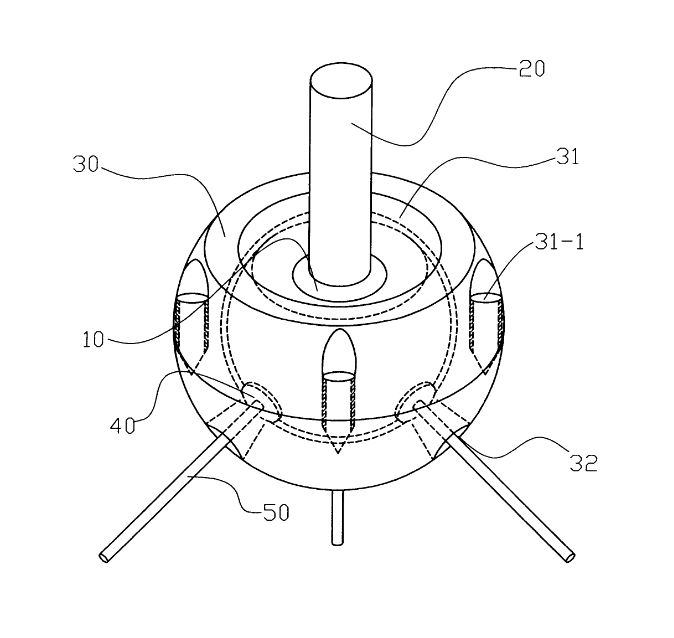
\includegraphics[width=0.5\textwidth]{figures/SongKwonKimImage.png}
    \caption[Song, Kwon, Kim, patent image.]{Song, Kwon, Kim, patent image.}
      \label{SongKwonKimImage}
\end{figure}


\subsection{Geometry}

\begin{figure}[H]
  \centering
  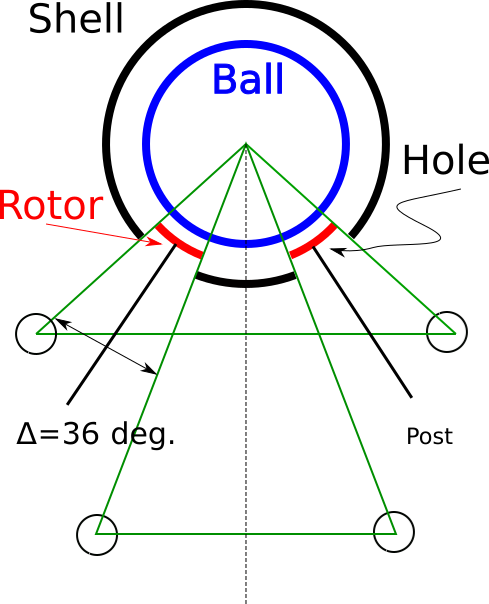
\includegraphics[width=0.5\textwidth]{figures/SimplifiedConstraintDrawing.png}
    \caption[Turret Joint Planar Geometry]{Turret Joint Planar Geometry}
      \label{simplified-constraint-drawing}
\end{figure}



"In fact it is a surprising result that we prove elsewhere \cite{readglussbot} in Appendix A that the maximum $Q$ which can be utilized
by an ideal turret joint happens to be
the famous golden ratio, $\varphi \equiv \frac{1 + \sqrt{5}}{2} \approx 1.618...$, and the maximum deviation for any one member coming
into the joint is $36\degree$."

 \begin{figure}[H]
  \centering
    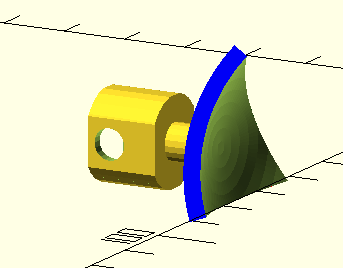
\includegraphics[width=0.5\textwidth]{figures/RotorModel.png}
    \caption[Triangular Rotor Model]{Triangular Rotor ModeL \emph{NEED TO UPDATE THIS FIGURE}}
      \label{rotormodel}
\end{figure}



" The Figure below shows most of the parts. The nylon triangular rotor is white and rests upon
 the red ball. The green part is a Tetrahelix lock, and the yellow parts are the locks for the Octet Truss
 geometry."

\begin{figure}[H]
  \centering
    \includegraphics[width=0.7\textwidth]{figures/Parts.jpg}
    \caption[3D Printed Parts]{3D Printed Parts \emph{NEED TO UPDATE THIS FIGURE}}
\end{figure}




\section{Placeholder for Photos}

\begin{figure}[H]
  \centering
    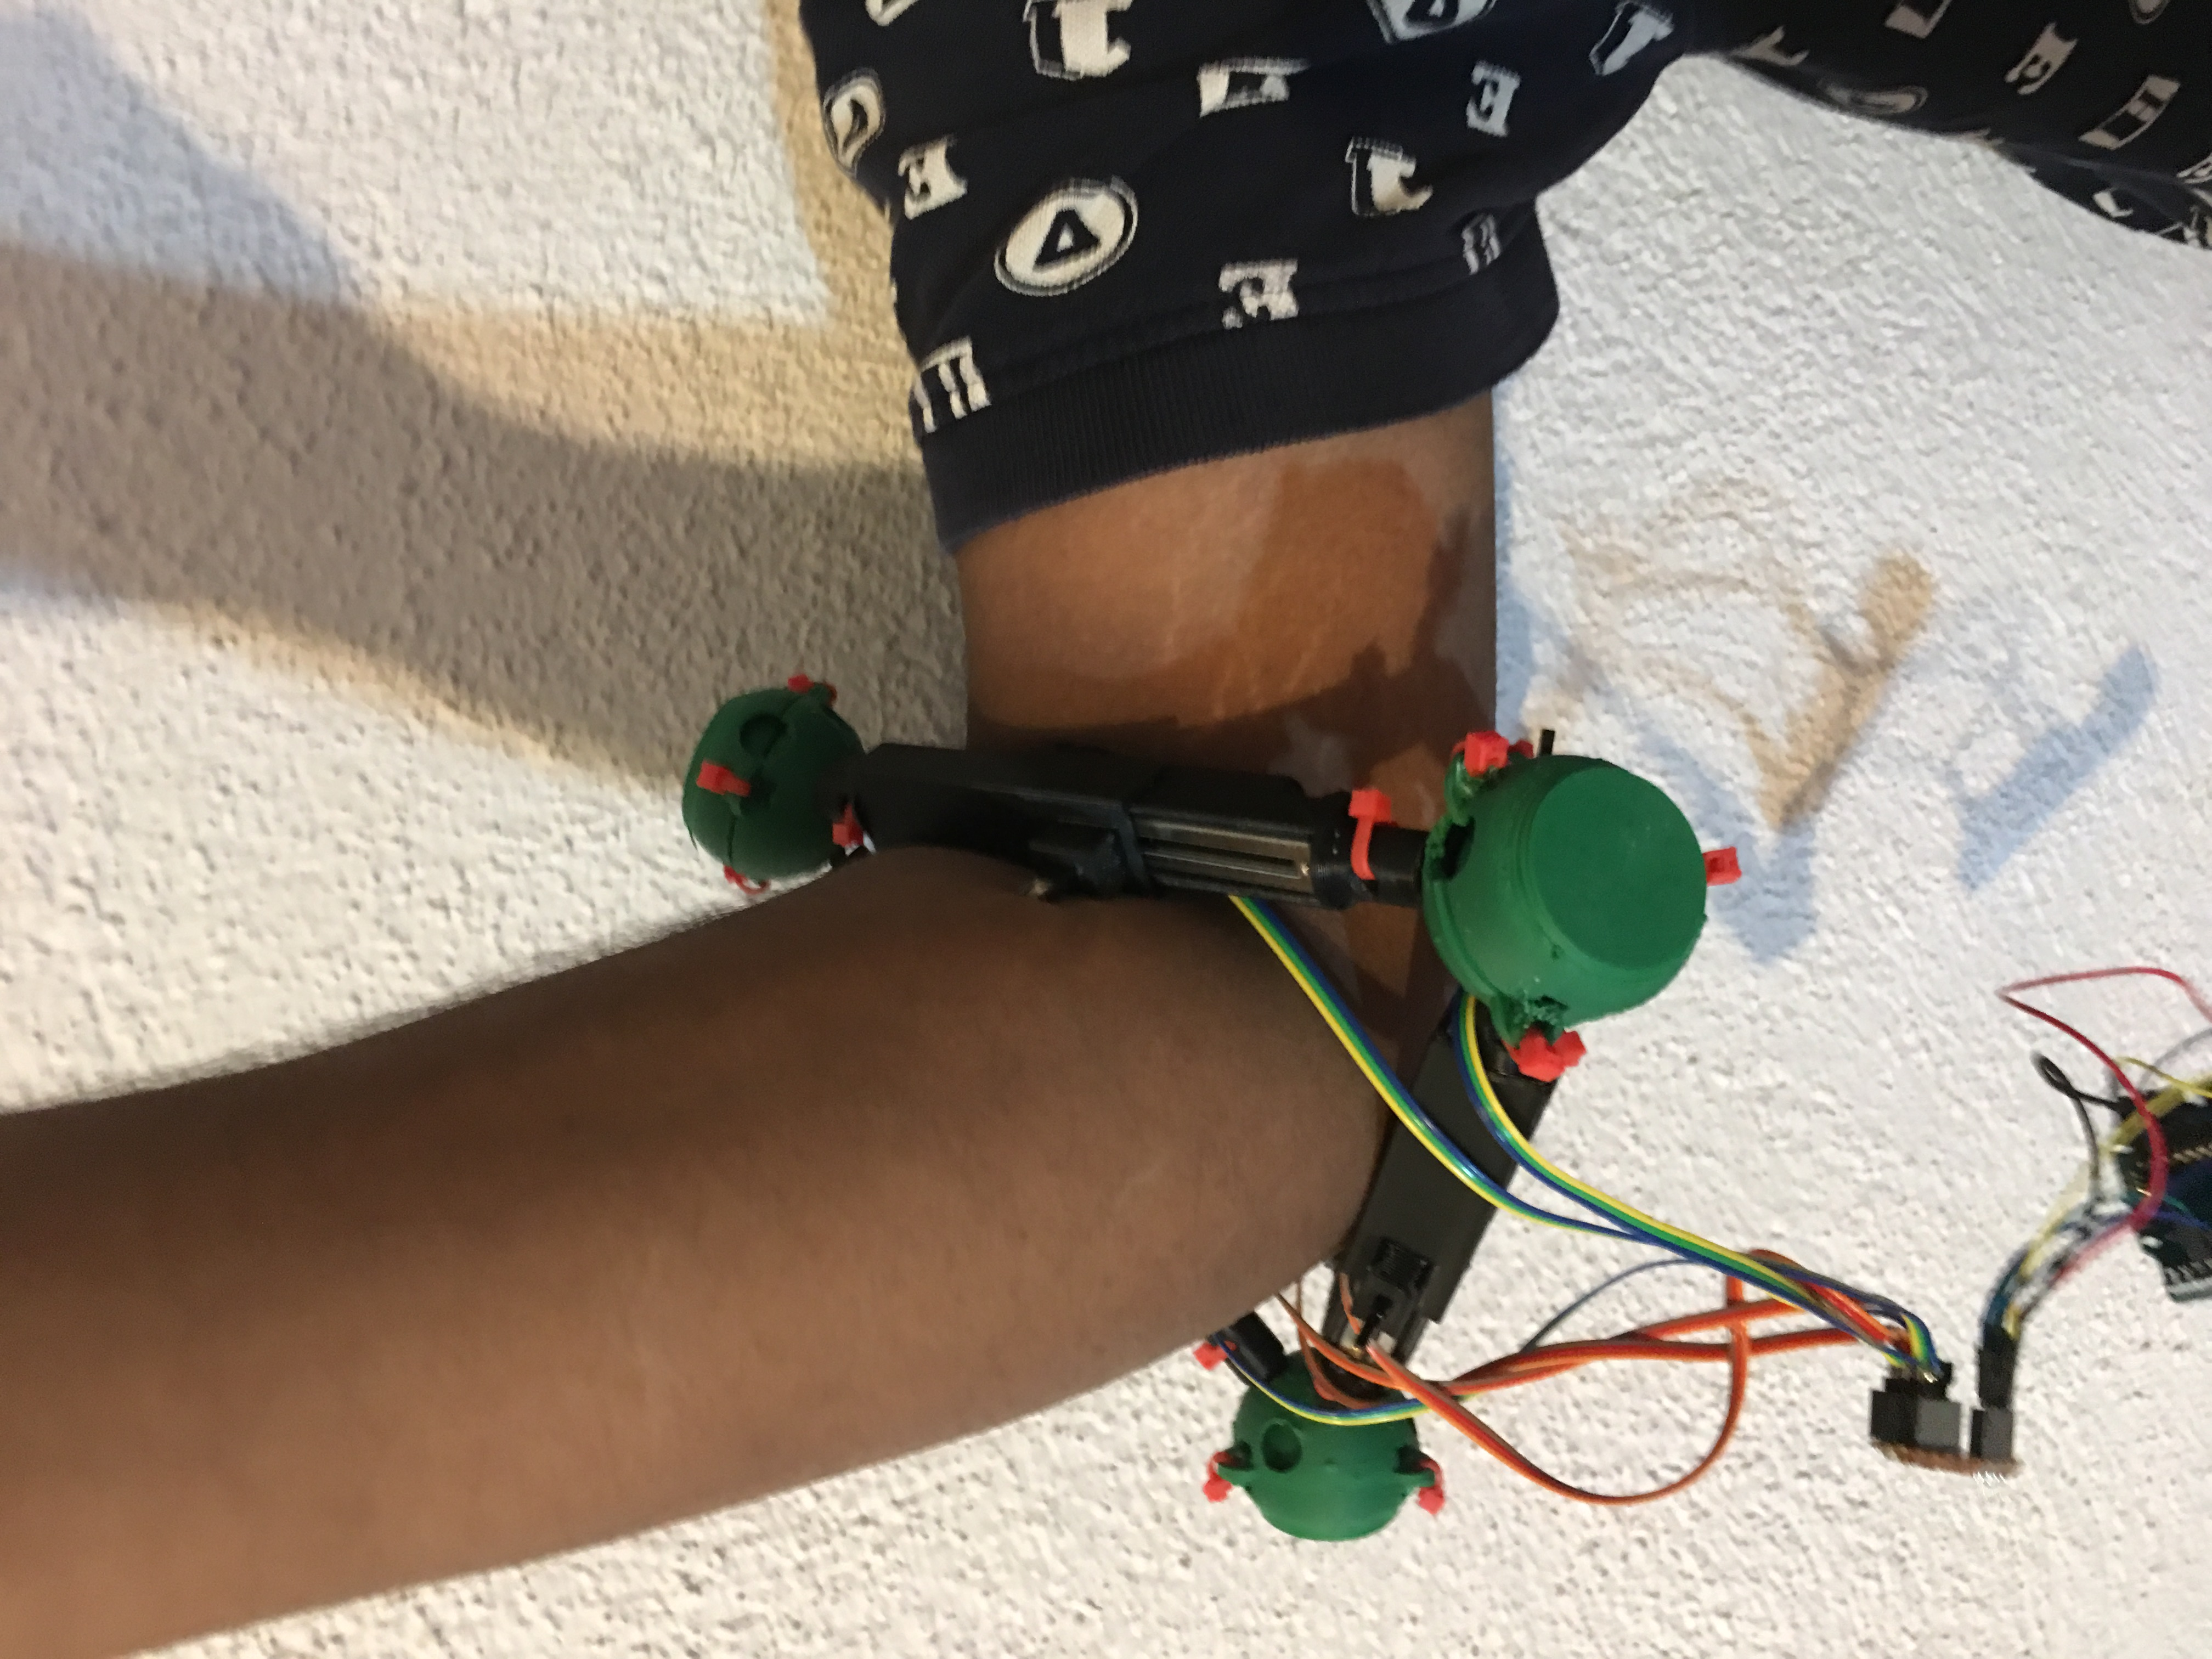
\includegraphics[angle=270,width=0.5\textwidth]{figures/ElbowFitting.JPG}
    \caption[One-tet controller fitting an elbow]{One-tet controller fitting an elbow}
      \label{fig:elbowfitting}
\end{figure}

\begin{figure}[H]
  \centering
    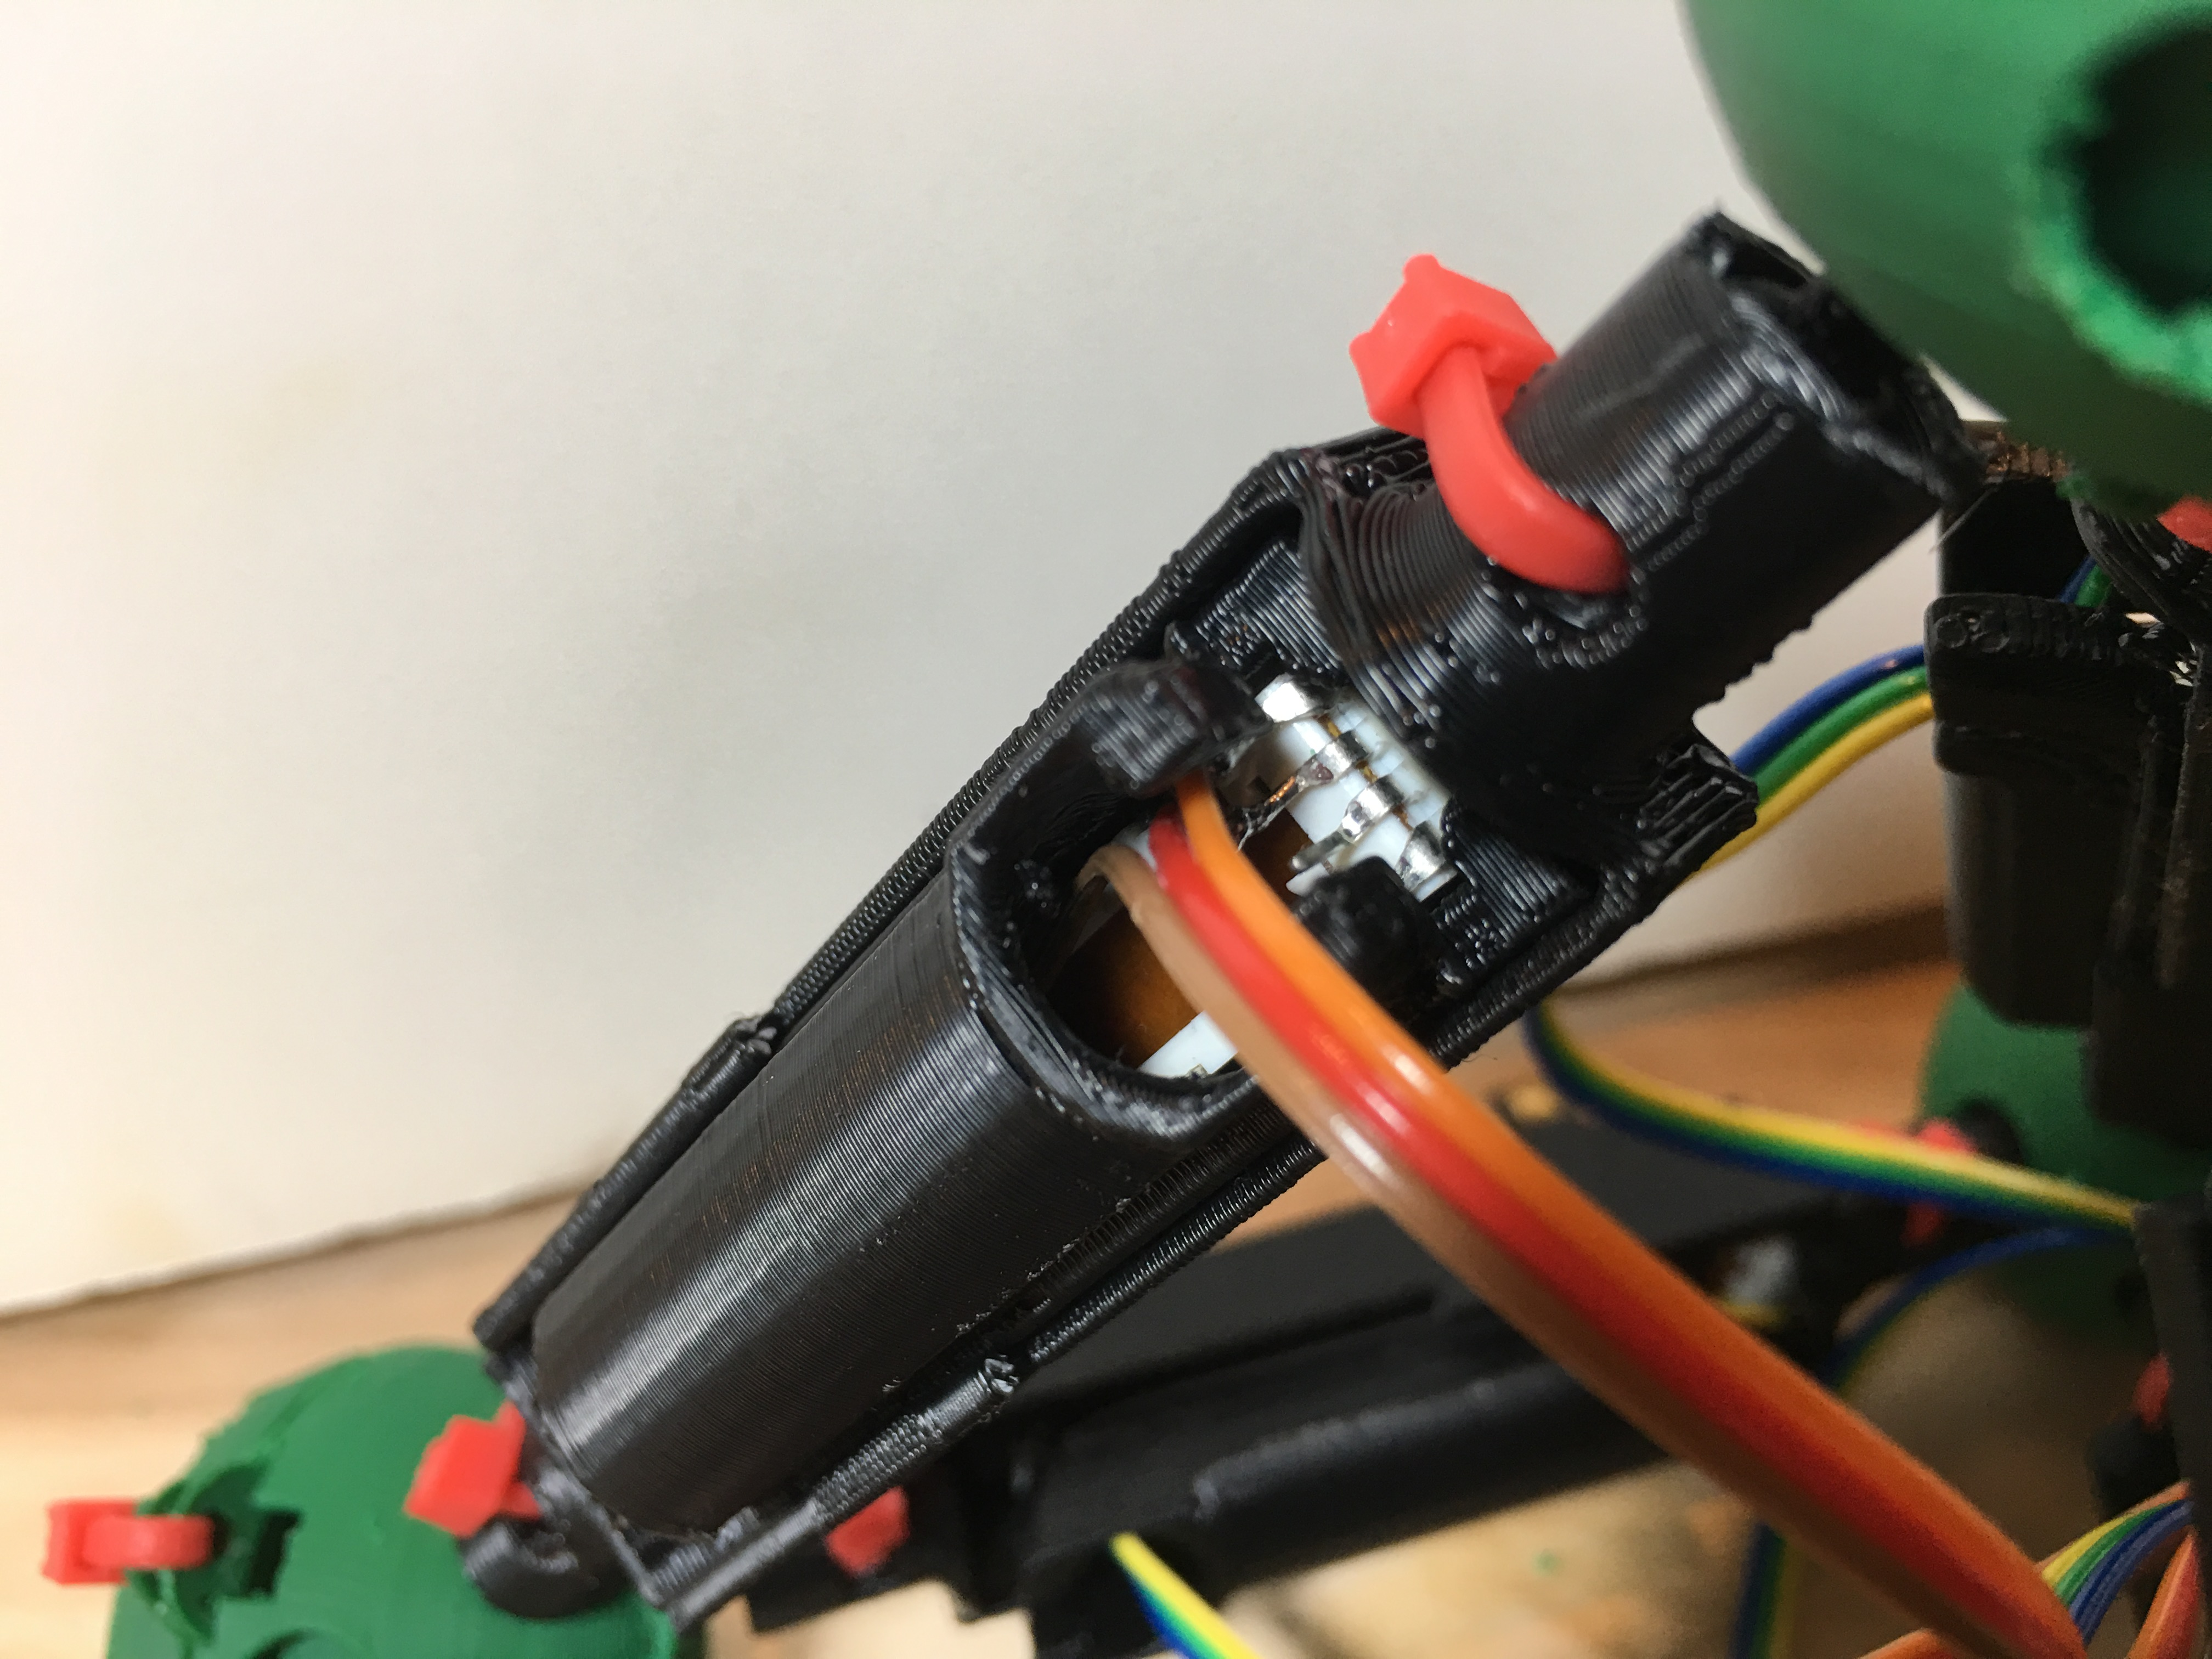
\includegraphics[width=0.5\textwidth]{figures/PotConnectionCloseUp.JPG}
    \caption[Close-up of Potentiometer Connection]{Close-up of Potentiometer Connection}
      \label{fig:potcloseup}
\end{figure}

\begin{figure}[H]
  \centering
    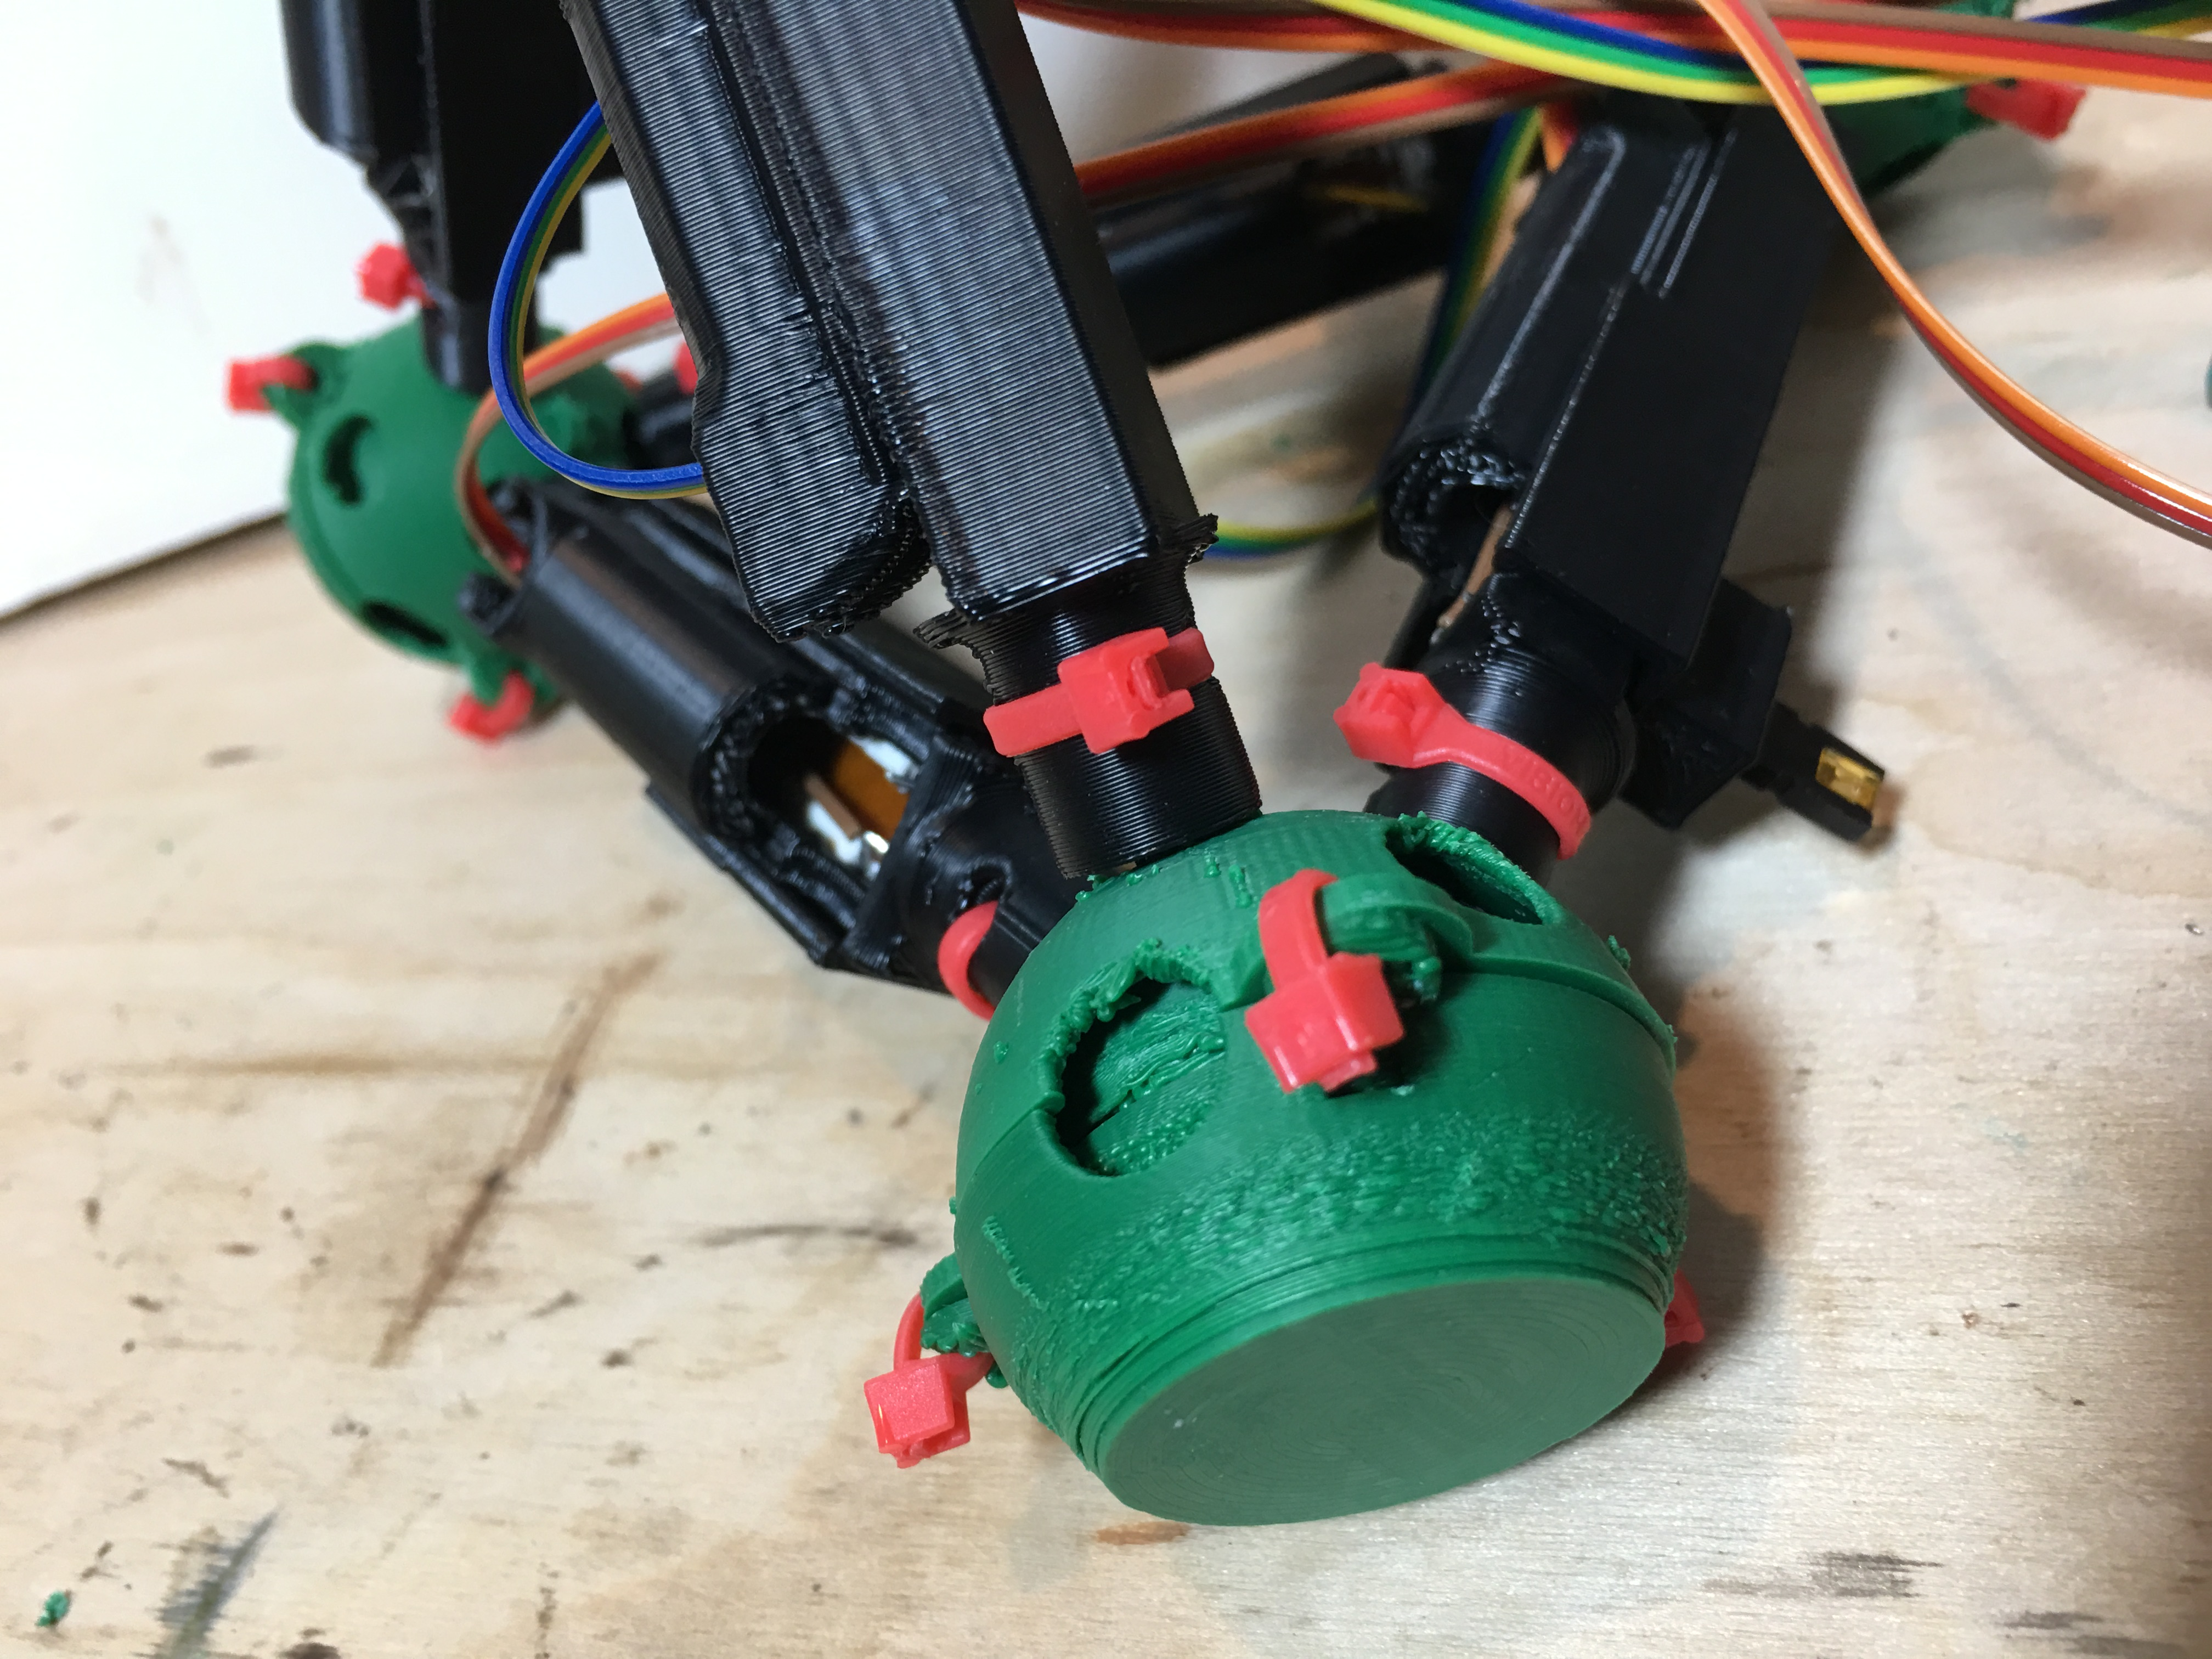
\includegraphics[width=0.5\textwidth]{figures/JointCloseUp.JPG}
    \caption[Joint Close Up]{Joint Close Up}
      \label{fig:jointcloseup}
\end{figure}

\begin{figure}[H]
  \centering
    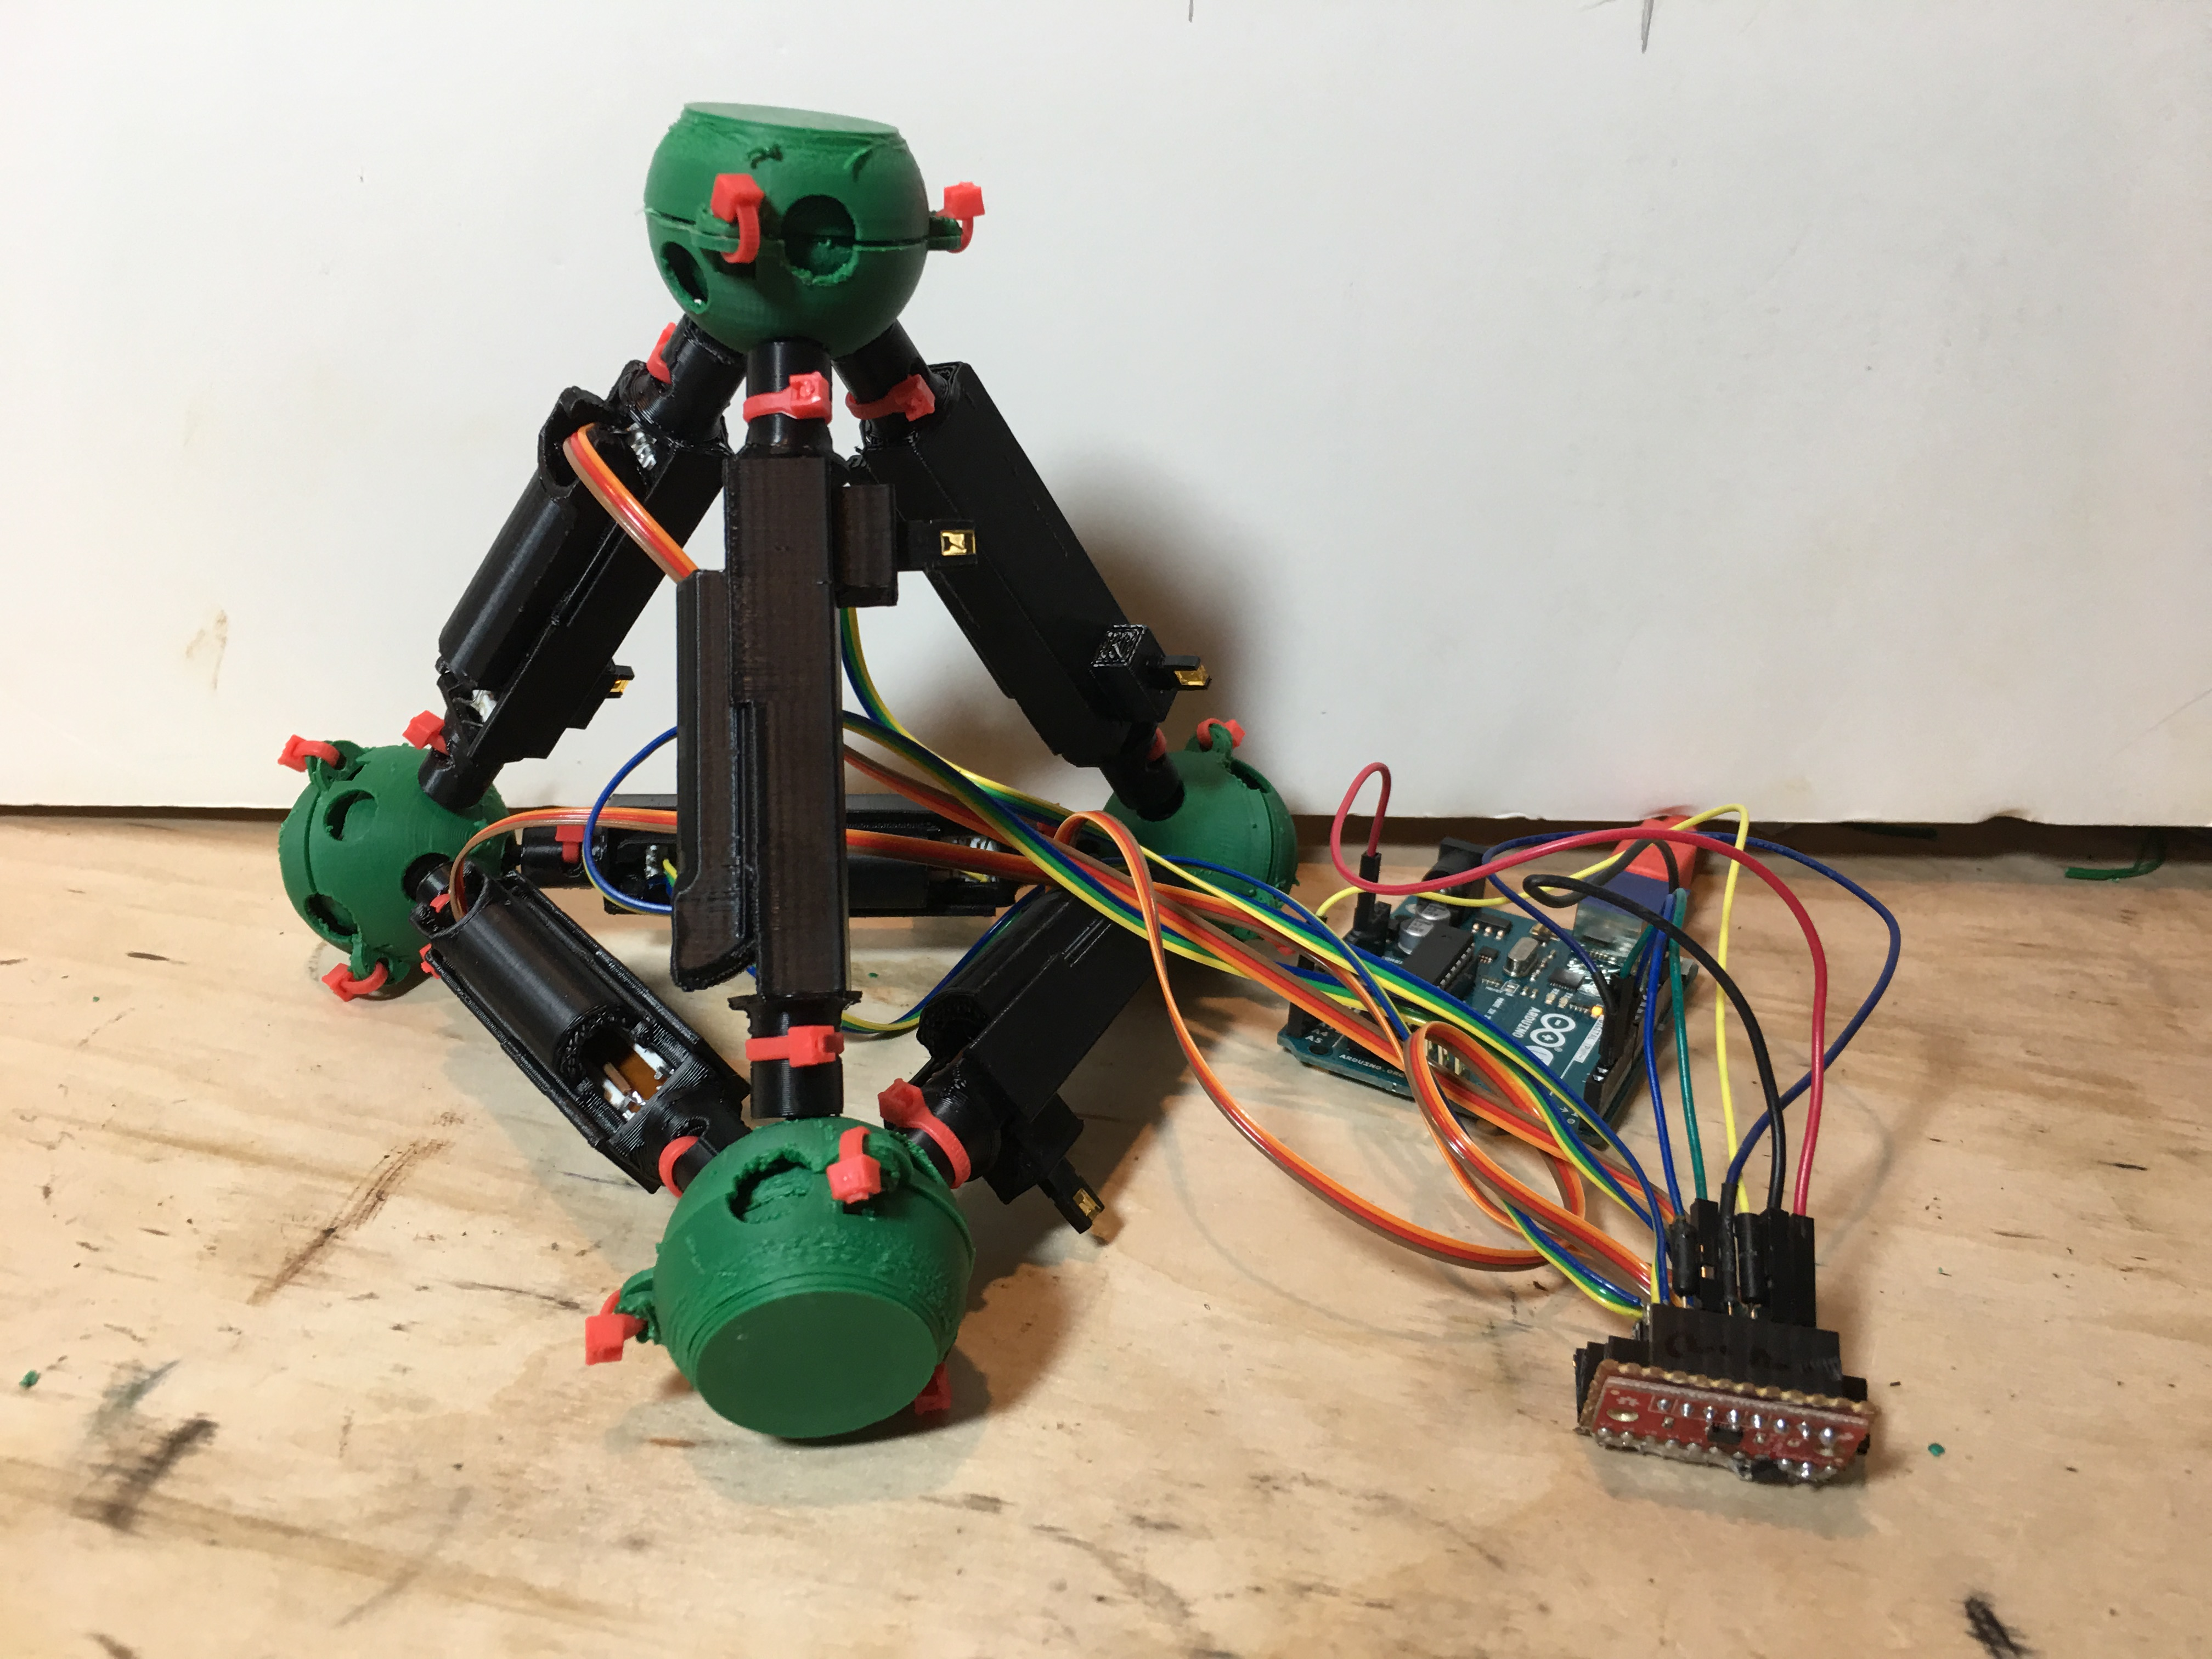
\includegraphics[width=0.5\textwidth]{figures/BasicOneTet.JPG}
    \caption[Basice One-Tet Controller]{Basic One-Tet Controller}
      \label{fig:basiconetet}
\end{figure}



\section{Future Steps}
\label{futuresteps}

\section{Contact and Getting Involved}

Public Invention
is a free-libre, open-source research, hardware, and software project that welcomes volunteers.
It is our goal to organize projects for the benefit of all humanity without seeking profit or intellectual property.
To assist, contact \href{mailto:read.robert@gmail.com}{$<$read.robert@gmail.com$>$}.

\bibliographystyle{plain}
\bibliography{gluss}

\end{document}
